\chapter{Implementation}
As evaluated in the last sections we will proceed to implement TF-DAC-MACS with small adaptions for a practical secure cloud storage system. To do so five entities need to implemented into our distributed system:  

\begin{itemize}
  \item \textbf{Central Server} does the initial setup of the global public parameter used in the later process. It publishes this information on a public bulletin board. Further, the CA is the central entry point to trigger and permit AA creations. It audits the \textit{Authority Identifier} (\ac{AID}) provided by the AA and which should be unique in this system. 

Further, the CA functions as a \textit{Certificate Authority}. It issues a certificate for the GID and RSA public keys of the user. This certificate can be revoked so that the user is not able to obtain new secret keys from the AA or other data owners.
The CA is also the central service that provides all necessary information to the client. Such as public attribute keys, encrypted user private attribute keys and certificates.
 The Central Server is honest-but-curious.
  \item \textbf{Attribute Authority (\ac{AA})} creates the secret keys for its attributes. Attributes are prefixed with the \ac{AID} to ensure uniqueness among the attribute universe. AAs are also untrusted but never collude with users. They have decryption power in their domain. 
  \item \textbf{Cloud Storage Provider (\ac{CSP})} The cloud storage provider provides storage to save the encrypted files. If an cipher text update is needed the CSP updates the cipher text accordingly. 
  \item \textbf{Users} download and decipher ciphertext. They receive attribute secret keys from the AA, GID and certificates from the server and two factor keys from the data owners. The CSP is honest-but-curious as well.
  \item \textbf{Data owner} are specifications of users who can issue two-factor keys to other users. The so called \textit{Two-Factor Key} (\ac{2FA}-Key), adds an additional security layer to the cipher text. It restricts the access to the encrypted plain text to a even smaller select user group.  
\end{itemize}

In the following sections, the different phases setup, encrypt, decrypt, attribute revocation and authentication key revocation are shortly explained. Please note that for any scheme details we referrer to the TF-DAC-MACS \cite{li2017two} paper .

\section{Setup}
\begin{figure}[!ht]
\centering
    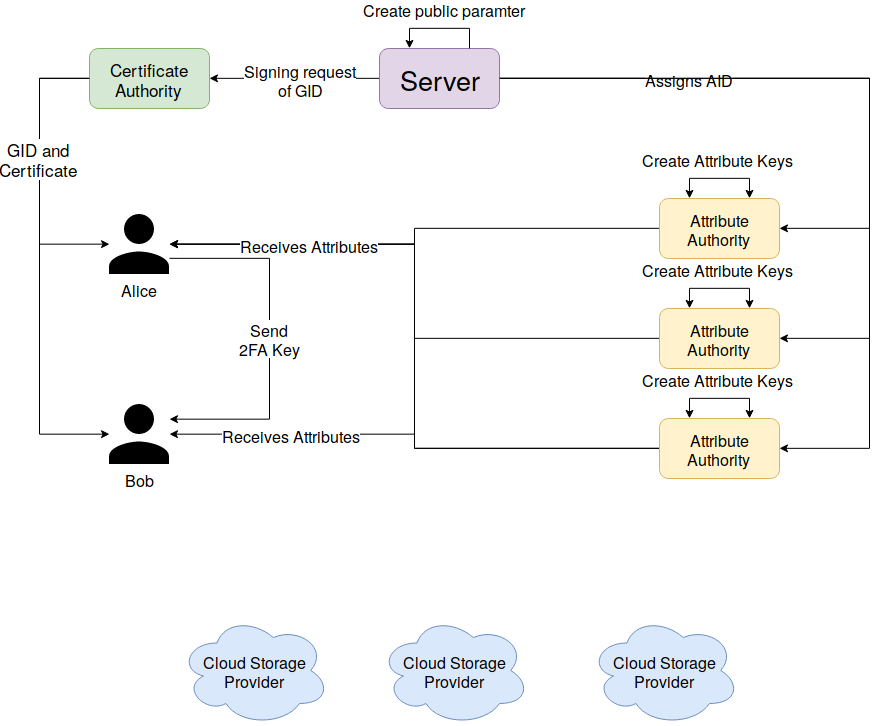
\includegraphics[width=\linewidth]{img/TF-DAC-MACS-overview-setup.png}
    \caption{Setup phase}
    \label{fig:tfdacmacs-setup}
\end{figure}

The setup summarizes the steps described in \cite{li2017two} such as: Setup, user registration, data owner registration, authority setup, key generation and authentication requests. 

The first step is to create the global public parameters on the server. Thous parameter are exposed on a public bulletin board and available for each entity in the system. Since they are required in every step it is assumed that the entity downloaded this information in advance. 

On AA setup the server first generates a new AID. This AID will be mapped to the domain name of this entity. So for example the TU-Berlin will have as its ID: "aa.tu-berlin.de". In this way it is ensured that no AID can double. Further, it would be verifiable via the certificate chain of TLS/SSL that this AID indeed belongs to the TU-Berlin. To do so the certificate coupled with this domain can be verified and then a query to "aa.tu-berlin.de" would lead to the corresponding AA of the TU-Berlin.

The AA is free to generate attribute keys. Attributes also have identifier and values assigned to them. Values and attribute identifier can be any valid string as long as it does not contain any special characters such as ":" or ".". The attribute will have the form of "<AID>.attr.<Attribute\_name>:<Attribute\_value>". For example the major computer science would be displayed as "aa.tu-berlin.de.attr.major:computer\_sience". Each attribute-value pair gets a secret key assigned. The public component for this attribute will be saved in the AA and published on the public bulletin board of the Central Server. 

In the next step, users are registered to the server. They receive the GID and a certificate for this GID. They can use the certificate later on to register to the AA or to authenticate them self to other users. The GID will be the email of the user. After the certificate is approved by the AA, it encrypts the user specific attribute value keys with the public key embedded in the presented certificate and pushes the encrypted attribute value keys to the central server. The user downloads and decrypts this keys. \todo{include registration flow graphic and describe this flow more deeply}

In the final setup, users can issue each other two factor keys so called \textit{authentication keys}. This authentication keys introduce a new layer of security where users can decide who exactly can decipher their plain text. In some cases this may be needed since access policies in ABE describe always a group of user and the exact members of this group remains hidden from the data owner.
 
An example flow to receive the 2FA-Key would look like this: If Bob wants to get an authentication key from Alice he sends an authentication request to the CA addressing Alice and containing his certificate. Alice gets notified about the request, checks the validity of the certificate and creates the authentication key for Bob. She  uses the public key embedded in Bobs certificate to encrypt the private authentication key and uploads it to the CA. Bob downloads the encrypted key and decrypts it. In the later manner, Bob can use this authentication key to authenticate against the cipher text created by Alice. 

The previous steps are summarized in the figure \ref{fig:tfdacmacs-setup}.

\section{Encryption}
\begin{figure}[!t]
\centering
    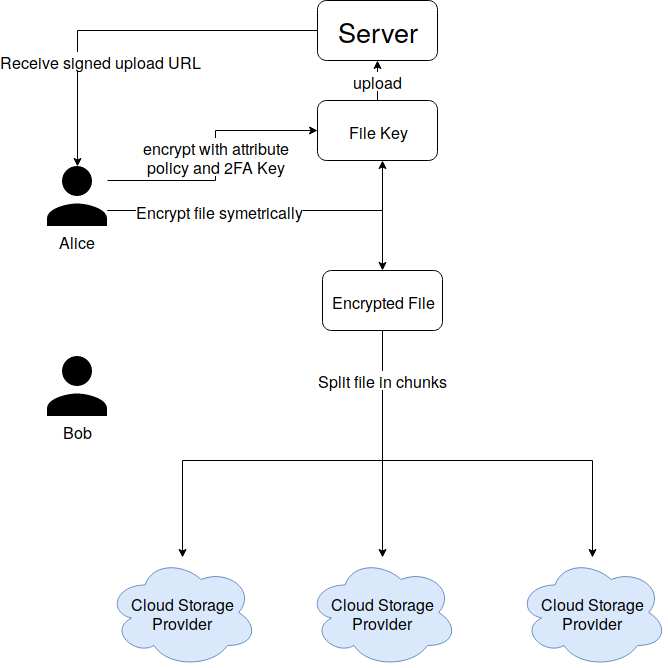
\includegraphics[width=0.7\linewidth]{img/TF-DAC-MACS-overview-encrypt.png}
    \caption{Encryption phase}
    \label{fig:tfdacmacs-encrypt}
\end{figure}

For en- and decryption we will still use the process of encrypting the file symmetrically to create a file key which will then encrypted under the attribute policy. This reduces the size of the content that will be encrypted with ABE to a minimum. Moreover, we can still benefit from the great performance of \ac{AES}. 

To upload a file encrypted under an access policy, Alice first creates the access policy (figure \ref{fig:tfdacmacs-encrypt}). In addition she is also able to encrypt the ciphertext with the authentication key she issued to Bob. \todo{Overwork graphic, might not match}. This results in a random secret $M \in G_T$. She transforms $M$ to a bit-stream and uses this as the key to encrypt the file content symmetrically. Alice uploads the ciphertext and the encrypted content to the CSP. 

\section{Decryption}
\begin{figure}[!t]
\centering
    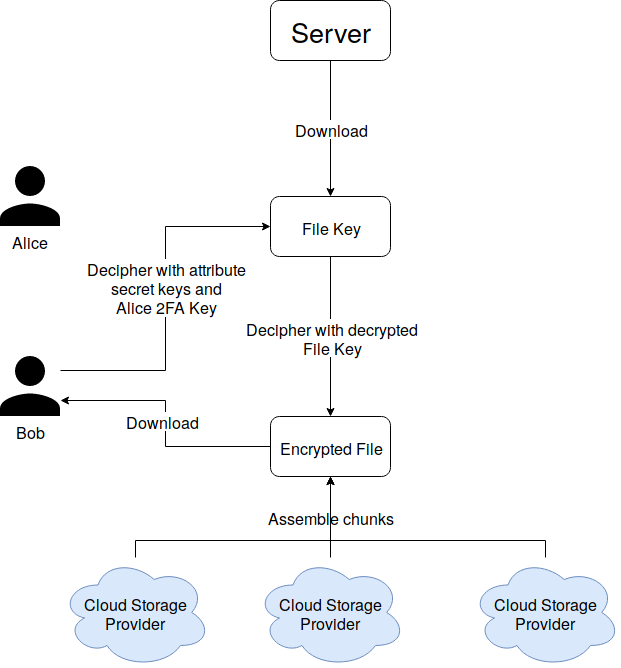
\includegraphics[width=0.7\linewidth]{img/TF-DAC-MACS-overview-decrypt.png}
    \caption{Decryption phase}
    \label{fig:tfdacmacs-decryption}
\end{figure}

On decryption first the ciphertext will be downloaded from the server. If Bob has a matching super set of attributes and the needed 2FA-Key he can recover the file key $m$ and transform it again to a bit-stream (figure \ref{fig:tfdacmacs-decryption})

Next, he downloads the encrypted file from the CSP and decrypts it with the recovered file key.

\section{Revoke attribute}
\begin{figure}[!t]
\centering
    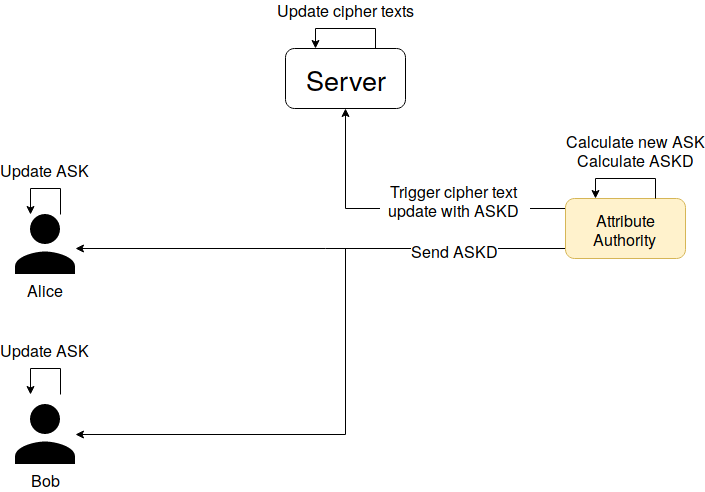
\includegraphics[width=0.7\linewidth]{img/TF-DAC-MACS-overview-revoce-attr.png}
    \caption{Attribute revocation}
    \label{fig:tfdacmacs-attr-revocation}
\end{figure}

As displayed in figure \ref{fig:tfdacmacs-attr-revocation}, a revocation of an attribute key is always triggered by the AA that administers this attribute. It first creates a new secret key for the revoked attribute and calculates for each user owning the old attribute a user-specific delta. This delta is send to each non-revoked user respectively. In addition, the AA calculates a cipher text update key. This is send to the CSP which then in turn starts updating all the cipher text for the new attribute secret key. This operation will not affect the plain text message in any kind. 

\section{Revoke two-factor key}
\begin{figure}[!t]
\centering
    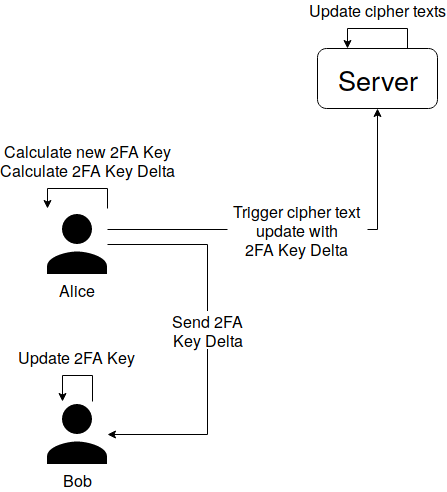
\includegraphics[width=0.6\linewidth]{img/TF-DAC-MACS-overview-revoce-user-key.png}
    \caption{Two-factor key revocation}
    \label{fig:tfdacmacs-user-auth-key-revocation}
\end{figure}

In a similar way as attributes are revoked, 2FA-Keys can be revoked. Alice, as the data owner, starts  by calculating a new two-factor key. She computes the delta to all old two-factor keys she issued and distributes them to all non-revoked users. Finally, she calculates the ciphertext update key and sends it to the CSP. The CSP updates all relevant cipher texts.

\section{Adaptions and Improvements}
While TF-DAC-MACS satisfy all the requirements it fits not perfectly. To make the scheme more usable, the fix contain that each cipher text need to be secured by a two-factor authentication was removed. In addition, the key generation of the attribute is made more dynamic. Now the attributes do not need to be known in the setup phase but can be created dynamically when an AA admin registers a user. Further, we propose a simple technique to break up TF-DAC-MACS n-of-n threshold policy in trade-off for performance. And finally we apply a technique proposed in \cite{bethencourt2007ciphertext} to implement numerical values and comparisons in boolean access formula. 

\subsection{Removing the fix two-factor contain}
To make \ac{TF-DAC-MACS} more practically applicable we removed the fixed two-factor constrain from the encryption, decryption, and cipher update phase. The two factor identifier $\alpha$ is used by the data owner to restrict the access to the content for certain users. 

This leads to the fact that the underlying \ac{ABE} schemes looses some of it expressiveness. The zero knowledge of the data owner on which individual is able to decrypt the cipher text is broken with the two factor part. Here each user, who wants to decrypt the encrypted content, needs to make an \textit{authentication request} to the data owner to receive the corresponding decryption key. To restore the possibility to let an unknown user group decrypt the cipher text, we make the two factor part optional. To do so we adapted encryption, decryption and cipher text update. The authentication key update will be ignored since it makes no sense to apply it on a non existing authentication key. 

\begin{itemize}
\item \textbf{Encryption:} 
We only need to update the $C_3$ part of the cipher text since it is the only one containing the two factor component $\alpha$.

The original $C_3$:
$$
C_3 = \Big( \prod_{v_{aid_{i}, j}\in W} g^{y_{aid_{i}, j}} \Big)^{s + \alpha} 
$$
is adapted to:
$$
\widehat{C}_3 = \Big( \prod_{v_{aid_{i}, j}\in W} g^{y_{aid_{i}, j}} \Big)^s
$$ 
In addition we will remove $oid$ from the ciphertext description since it referrers to the data owner ID which is only needed on authentication key update.

\item \textbf{Decryption:}
$SK_W = \prod_{v_{aid_i,j} \in W} SK_{v_{aid_i,j}}$ and $UPK_W = \prod_{v_{aid_i,j} \in W} UPK_{v_{aid_i,j}}$ remain defined in the same was as defined in the paper. 

On decryption the user does not need to generate $UPK_W$ and $SK_{uid, oid}$ anymore. The decryption equation is updated to:

$$
m = \frac{C_1 \cdotp e(H(uid), \widehat{C}_3)}{e(C_2, SK_W)}
$$

Note that the original decryption equation results in the above equation when the two factor part is deducted.

\begin{equation}
\begin{split}
m &= \frac{C_1 \cdotp e(H(uid), C_3)}{e(C_2, SK_W)e(SK_{uid, oid}, UPK_W)} \\
  &= \frac{C_1 \cdotp e\Big(H(uid), \Big( \prod_{v_{aid_{i}, j}\in W} g^{y_{aid_{i}, j}} \Big)^{s + \alpha} \Big)}{e(C_2, SK_W)e(H(uid)^\alpha, \prod_{v_{aid_i,j} \in W} UPK_{v_{aid_i,j}})} \\
  &= \frac{C_1 \cdotp e\Big(H(uid), \Big( \prod_{v_{aid_{i}, j}\in W} g^{y_{aid_{i}, j}} \Big)^{s + \alpha} \Big)}{e(C_2, SK_W)e(H(uid)^\alpha, \prod_{v_{aid_i,j} \in W} g^{y_{aid_i,j}})} \\
  &= \frac{C_1 \cdotp e\Big(H(uid), \Big( \prod_{v_{aid_{i}, j}\in W} g^{y_{aid_{i}, j}} \Big) \Big)^{s + \alpha}}{e(C_2, SK_W)e(H(uid), \prod_{v_{aid_i,j} \in W} g^{y_{aid_i,j}})^\alpha} \\
  &= \frac{C_1 \cdotp e\Big(H(uid), \Big( \prod_{v_{aid_{i}, j}\in W} g^{y_{aid_{i}, j}} \Big) \Big)^{s}}{e(C_2, SK_W)} \\
  &= \frac{C_1 \cdotp e\Big(H(uid), \Big( \prod_{v_{aid_{i}, j}\in W} g^{y_{aid_{i}, j}} \Big)^{s} \Big)}{e(C_2, SK_W)} \\
  &= \frac{C_1 \cdotp e(H(uid), \widehat{C}_3)}{e(C_2, SK_W)}
\end{split}
\label{eq:2faRemoval}
\end{equation}

As shown, no security is threatened since we end up at the same equation as we would if we had the two factor part included. 

\item \textbf{Attribute revocation:}
The cipher text update key is adapted from

$$
CUK^{ID_W}_{v_{aid_i,j}} = (g^s \cdotp g^\alpha)^{y'_{aid_i,j} - y_{aid_i,j}}
$$

to 

$$
\widehat{CUK}^{ID_W}_{v_{aid_i,j}} = (g^s)^{y'_{aid_i,j} - y_{aid_i,j}}
$$

$\widehat{C}'_3$ now computes as 

\begin{equation}
\begin{split}
\widehat{C}'_3 &= \widehat{C}_3 \cdotp \widehat{CUK}^{ID_W}_{v_{aid_i,j}} \\
&\cdotp \Big( \prod_{v_{aid_{t}, j}\in W, v_{aid_t, j} \neq v_{aid_i,j}} g^{y_{aid_{i}, j}} \Big)^{r} \cdotp (g^{y'_{aid_i,j}})^{r} \\
&= \Big( \prod_{v_{aid_{t}, j}\in W, v_{aid_t, j} \neq v_{aid_i,j}} g^{y_{aid_{i}, j}} \Big)^{s + r} \cdotp (g^{y'_{aid_i,j}})^{s + r}
\end{split}
\end{equation}

It can be shown that $C'_3$ computes to the message $m$ in the same way as shown in equation \ref{eq:2faRemoval}.

\item \textbf{Authentication update:}
Nothing need to change since cipher text do not contain authentication components. 
\end{itemize}

\subsection{Dynamic Secret Key Generation}
Another small adaptation in the \ac{TF-DAC-MACS} scheme was that the attributes for each \ac{AA} does not have to be known on AA initialization. They can as well be created on each users key generation. This reduces the universe of possible attribute values to thous who are actually needed.

\section{Extension To DNF-Policy}
One big advantage of TF-DAC-MACS is its constant size cipher text. It archives this by only allowing n-of-n threshold policy. This means that a data owner is only allowed to create \textit{AND} policies to encrypt his content. However, extending this scheme to n-of-m threshold policy is not trivial. To not break any security constrains we decided to just upload multiple versions of the same cipher text encrypted under different policies. Now, an user only needs to decipher one version of the cipher text to recover the encrypted content. 

Using this approach we enable access policies in disjunctive normal form (DNF) for the trade-off of linear cipher text overhead and linear overhead on cipher text updates (both scaling with the number of disjunctions).

\section{Numerical Attributes}
As described in \cite{bethencourt2007ciphertext} we could display numeric values in binary. Each number $x$ is composed of $\lceil log_2(x) \rceil$ attributes. Each of this attributes relate to either a $1$ or $0$ in one position in the binary number representation of $x$. So for example the number $5$ in binary would be displayed as $0101$ and its attribute would be: $x:0***$, $x:*1**$, $x:**0*$ and $x:***1$. 

If a user now wants to create a policy where he challenges a number $x$ to be greater or equal to $3$ he creates a policy: "$(x:1*** or (x:*1** or (x:**1* and x:***1))$". Analogous the policy for $x$ smaller than $4$: "$(x:0*** and (x:*0** or (x:*1** and x:**0* and x:***0))$".

Disadvantage of this representation is that it is limited in space. To display a 32-bit number we must issue 64 attribute values and maintain 64 attribute value keys. 


\section{Technologies}
To develop the first prototype of the system defined previously we will use the following technology stack:

\begin{itemize}
  \item \textbf{Spring boot}
  \item \textbf{Docker}
  \item \textbf{jPBC} \cite{ISCC:DecIov11}
  \item \textbf{...}
\end{itemize}
\todo{write me}

\section{Problems}

\subsection{En- and decrypting arbitrary data}
TF-DAC-MACS takes as an input for encryption a message $M \in GT$. Since there is not easy way to reconstruct a message from an element in $G_T$, we have to combine some encryption techniques to encrypt arbitrary data. 

The algorithm first chooses a random $M \in GT$ and outputs $M$ together with the constructed cipher text. $M$ is then hashed into a byte buffer using \ac{SHA}-256. In the next step we will encrypt our arbitrary data using \ac{AES} and as the key the previous computed hash. 

On decryption we first reconstruct $M$ using the ABE decryption technique and then hashing $M$ again to reconstruct our AES secret key. 